\documentclass[a4paper, 12pt]{article}
\usepackage[slovene]{babel}
\usepackage[utf8]{inputenc}
\usepackage[T1]{fontenc}
\setlength{\parindent}{0px}
\setlength{\parskip}{10px}
%standard

\usepackage{listings}
\usepackage{color}
\usepackage{amssymb}
\usepackage{tikz}
\usepackage{pgfplots}
\usetikzlibrary{patterns}
\pgfplotsset{width=7cm, compat=1.10}
\usepgfplotslibrary{fillbetween}

\title{Avditorne vaje za Programiranje II}
\author{Matej Blagšič}

\begin{document}
%--------------------------------------------
\definecolor{dkgreen}{rgb}{0,0.6,0}
\definecolor{gray}{rgb}{0.5,0.5,0.5}
\definecolor{mauve}{rgb}{0.58,0,0.82}
\definecolor{lgray}{RGB}{250,250,250}
%--------------------------------------------
	\lstset{
		frame=l,%single
		language=C,
		aboveskip=3mm,
		belowskip=3mm,
		showstringspaces=false,
		columns=flexible,
		basicstyle={\small\ttfamily},
		numbers=none,
		numberstyle=\tiny\color{gray},
		keywordstyle=\color{blue},
		commentstyle=\color{dkgreen},
		stringstyle=\color{mauve},
		breaklines=true,
		breakatwhitespace=true,
		tabsize=4,
		backgroundcolor=\color{lgray},
		moredelim=**[is][\color{dkgreen}]{@}{@}
	}
%-------------------------------------------

%-------------------------------------------
	\maketitle
	\thispagestyle{empty}
	\pagebreak
	\setcounter{page}{1}
	\tableofcontents
	\pagebreak
%-----------------------------------Tu naprej

\section{Prva vaja}

\section{Druga vaja}

\underline{Izračunaj $\int_{x_0}^{x_1}\, 2x^2-5x\, dx$. Rezultat preveri analitično.}	\

Če analitično integriramo itegral, dobimo: $\int_{x_0}^{x_1}\, 2x^2-5x\, dx = 2\frac{x_1^3}3-5\frac{x_0^2}2$\

Sedaj spišimo kodo:
\begin{lstlisting}
int main(){
	float x, x0, x1;
	float dx = 0.0000001;
	float integral = 0;
	printf("vnesi spodno mejo");
	scanf("%f",&x0);
	printf("Vnesi zgornjo mejo");
	scanf("%f",&x1);

	for(x=x0; x<x1;x+=dx){
		integral += dx*(2*x*x-5*x);
	}

	printf("Integral znasa: %f\n", integral);
	return 0;
}
\end{lstlisting}
Pri programu nam spremenljivka dx sporoči, kako širok del območja integrira. Manjša, kot je cifra, bolj natančno izračuna. x0 in x1 sta spodnja in zgornja meja integracije, x pa je spremenjivka, ki jo premikamo po intervalu za dx razdaljo in seštevamo pravokotnike.
	
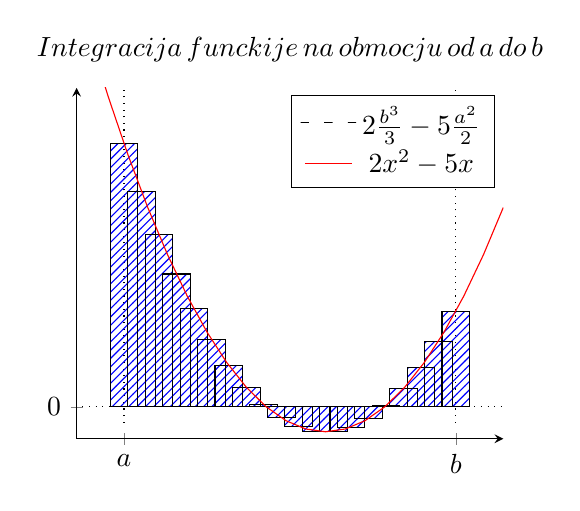
\begin{tikzpicture}
\begin{axis}[axis lines=left,xmin=-4,xmax=5,ymin=-4,ymax=40,ytick={0}, yticklabel={$0$},xtick={-3,4},xticklabels={$a$,$b$},title={$Integracija\, funckije\, na\, obmocju\, od\,a\, do\, b$}]

\addplot[dotted]{0};
\addplot+[mark=none, dotted, color=black] coordinates {(-3, -2)(-3,40)};
\addplot+[mark=none, dotted, color=black] coordinates {(4, -2)(4,40)};
\addplot[domain=-3:4,ybar, samples=20, pattern = north east lines, pattern color=blue]{2*x*x-5*x}\closedcycle;
\addplot[color = red]{2*x*x-5*x};
\legend{,,,$ 2\frac{b^3}3-5\frac{a^2}2$, $2x^2-5x$}

\end{axis}
\end{tikzpicture}
	
\section{Tretja vaja}
\subsection*{1. naloga}

\underline{Napiši program, ki izpiše in izračuna faktorielo(fakulteta) nekega števila(1-20)}\

Pri temu programu spoznamo omejitve velikosti spremenljivk. Pomemno je, da so števila, ki jih hočemo hraniti in predstavljani v polni natančnosti ne presegajo velikosti spremenljivke. Če ne, potem se prične pačenje podatkov. Vidimo, da lahko uporabimo izrad long long in s tem povečamo obseh navadnega long tipa. Podobno lahko naredimo tudi s spremenljivkam s plavajočo vejico, recimo \lstinline|long double|.
\begin{lstlisting}
int main(){
	unsigned long long resitev = 1, n;

	for(n=1; n<=20; n++){
		for(int i=1; i<=n; i++){
			resitev *= i;
		}
		printf("Faktoriela od %lld! je %lld\n", n, resitev);
		resitev = 1;
	}
	return 0;
}
\end{lstlisting}

\subsection*{2. naloga}
	
\underline{Napiši program, ki sešteje maso lune in zemlje ter sonca.}\

Namen vaje je dodatno spoznati omejitve spremenljivk v programskem jeziku C. Mase lune, zemlje in sonca so ogromne, zato se začenja poznati popačenje podatkov. Ugotovili smo, da dobimo kar se da dobre rezultate, če uporabimo \lstinline|double|, ki ima največji obseh, a se vseeno na določenem mestu pojavi naključna številka, ki ni podana med vhodnimi podatki.

\begin{lstlisting}
int main(){
	double luna = 7.348e22;
	double zemlja = 5.972e24;
	double sonce = 1.989e30;
	
	printf("Masa lune je: %40.0lf \n",luna);
	printf("Masa zemlje je: %40.0lf \n",zemlja);
	printf("Masa sonca je: %40.0lf \n",sonce);
	printf("Skupna masa je: %40.0lf\n", zemlja+luna);
	printf("Skupna masa sonca pa lune je: %40.0lf\n", sonce+luna);
	
	return 0;
}
\end{lstlisting}
	
	
	
	
	
\end{document}